\documentclass{article}

% ==========================================================
%  Pacchetti importati
% ==========================================================
\usepackage[italian]{babel}
\usepackage[letterpaper,top=2cm,bottom=2cm,left=3cm,right=3cm,marginparwidth=1.75cm]{geometry}
\usepackage{amsmath}
\usepackage{graphicx}
\usepackage{subcaption}
\usepackage{textcomp}
\usepackage{float}
\usepackage{ragged2e}
\usepackage[export]{adjustbox}
\usepackage[table, dvipsnames]{xcolor}
\usepackage{tcolorbox}
\usepackage{tabularx}
\usepackage{fancyhdr}
\usepackage{lastpage}
\usepackage[labelfont=bf, font=small]{caption}
\usepackage{pifont}

% ==========================================================
% Informazioni pdf
% ==========================================================
\usepackage[colorlinks=true, allcolors=blue,
            pdfauthor={Matteo Drago},
            pdftitle={Bivacco di Barc},
            pdfsubject={Diario bivacchi e trekking},
            pdfkeywords={bivacco, montagna, trekking, diario},
            pdfproducer={LaTeX},
            pdfcreator={TeX Live 2025},
            pdflang={it-IT},
            pdfdisplaydoctitle=true,
            pdfstartview=FitH,
            pdfpagemode=UseOutlines]{hyperref}
                
\title{\textbf{Bivacco di Barc - 1918 m s.l.m}}
\author{Matteo Drago}

% ==========================================================
% Impostazioni per header e footer in ogni pagina
% ==========================================================
\pagestyle{fancy}
\fancyhf{} % Pulisce tutti i campi di intestazione e piè di pagina
\fancyhead[R]{
\includegraphics[height=1.5cm]{images/toothless.jpeg}} % Posiziona il logo a destra (R) nell'intestazione
\fancyfoot[C]{\small\itshape Bivacco di Barc - Aprile 2026}
\fancyfoot[R]{Pagina \thepage\ di \pageref{LastPage}} % lato destro
\renewcommand{\headrulewidth}{0pt} % Rimuove la linea orizzontale nell'intestazione (opzionale)

%==========================================================

\begin{document}
\maketitle
\thispagestyle{fancy} % Aggiungi questa riga

% ==========================================================
%  Abstract
% ==========================================================
\begin{abstract}
Questo documento raccoglie e organizza le informazioni che ho acquisito nel corso degli anni sui bivacchi, basate sulle mie esperienze dirette. Sebbene non si proponga come una guida esaustiva e perfetta, offre il minimo indispensabile per una buona vita in bivacco, con consigli pratici e diretti per chiunque desideri affrontare al meglio queste pazze ma piacevoli avventure.
\end{abstract}

\section{Il bivacco}

% ==========================================================
% Immagine a sinistra, testo a destra allineato in alto
% ==========================================================
\noindent
\begin{minipage}[t]{0.45\textwidth}
  \vspace{0pt} % forza l'allineamento in alto
  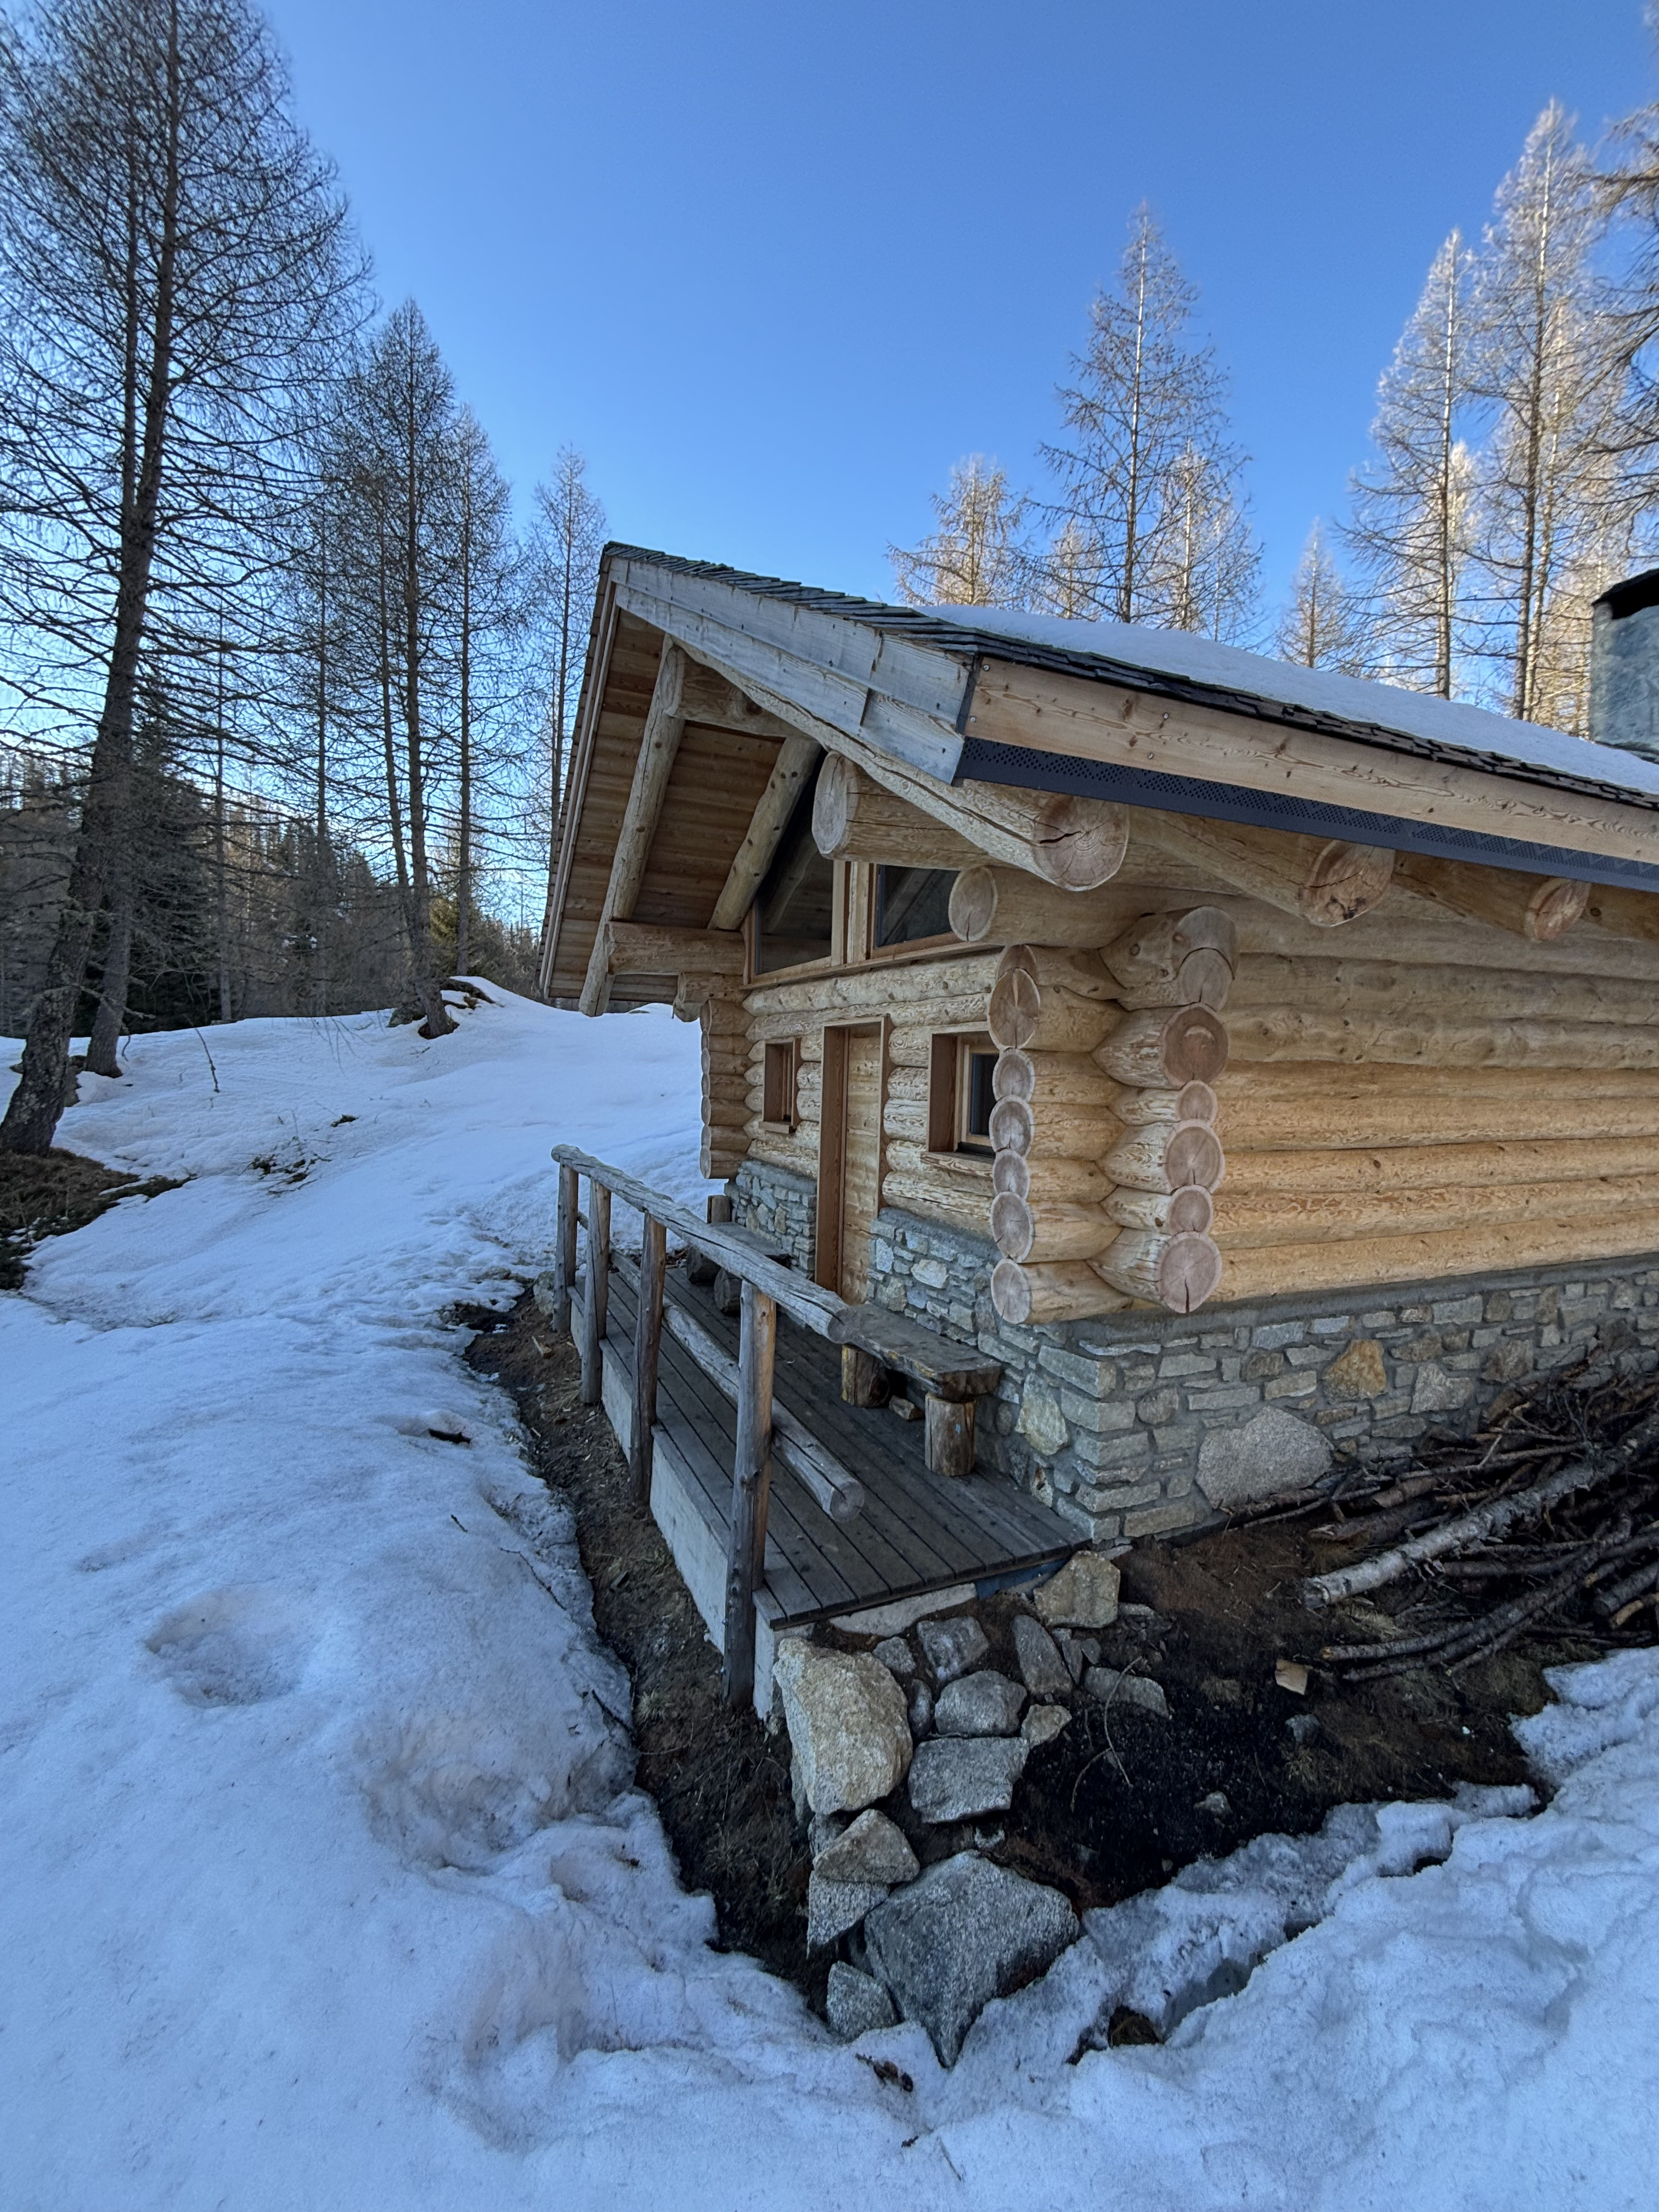
\includegraphics[width=\linewidth, frame]{images/bivacco.jpg}
\end{minipage}%
\hfill
\begin{minipage}[t]{0.5\textwidth}
  \vspace{0pt} % forza l'allineamento in alto

  Regione\\
  \textbf{\large Trentino-Alto Adige}
  \\[1em] % Aggiunge una riga vuota qui
  Provincia/Comune\\
  \textbf{\large Trento / Vermiglio}
  \\[1em] % Aggiunge una riga vuota qui
  Gruppo montuoso\\
  \textbf{\large Gruppo della Presanella}
  \\[1em] % Aggiunge una riga vuota qui
  Quota\\  
  \textbf{\large 1918 m s.l.m.}
  \\[1em] % Aggiunge una riga vuota qui
  Coordinate\\
  \textbf{\large \href{https://maps.google.com/?q=46.274987,10.708379}{46.274987° N, 10.708379° E}}
  \\[1em] % aggiunge una riga vuota qui
  Apertura\\  
  \textbf{\large Non gestito, sempre aperto}

\end{minipage}

\subsection{Caratteristiche}
Il bivacco Barco è stato costruito di fronte al lago di Barco, andando a sostituire un vecchio rudere.
Il bivacco è caratterizzato da:
\begin{itemize}
\item \textbf{Piano terra}: prevede la presenza di una stufa economica, un tavolo e un armadio fornito di materiale vario.
\item \textbf{Piano superiore}: costituito da un soppalco spazioso con materassi che offrono la possibilità di pernottare ad una decina circa di persone.
\item \textbf{Spazio esterno}: sui lati del bivacco si trovano scorte di legna e, sparsi nella zona, ci sono diversi tavoli e spazi per fare il fuoco.
\end{itemize}

\section{Come ci siamo arrivati}
Siamo partiti dal centro del paese di Vermiglio, addentrandoci fin da subito in un sentiero immerso nella natura incontaminata. In breve tempo si raggiunge la \href{https://maps.google.com/?q=46.290830,10.729838}{malga del Dosso} (anch'essa aperta), che offre un ottimo punto di riposo a metà percorso, oltre a una splendida vista sulla valle sottostante. Superata la malga, si raggiunge il bivacco senza particolari difficoltà.
Il giorno successivo abbiamo proseguito lungo il giro ad anello per fare ritorno a Vermiglio.


\begin{figure}[H]
    \centering
    % Colonna di sinistra, allineata in alto
    \begin{subfigure}[t]{0.45\textwidth}
        \centering
        \vspace{0pt} % Forziamo l'allineamento in alto
        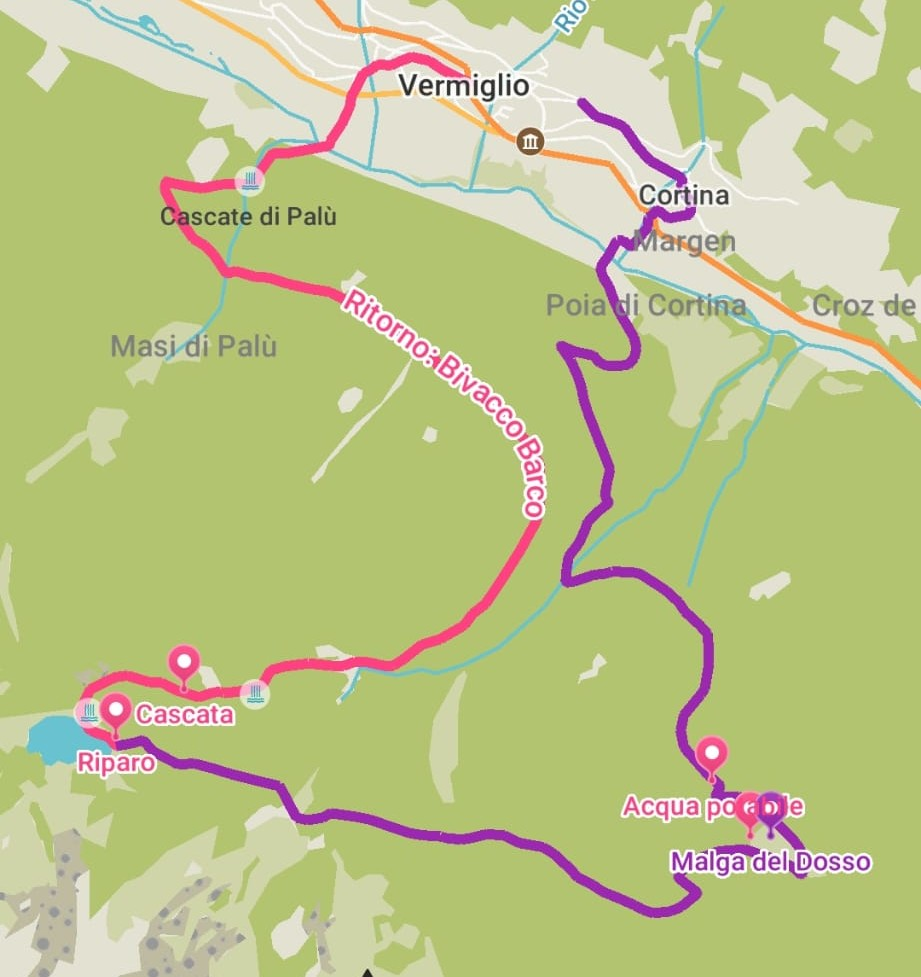
\includegraphics[width=\textwidth]{images/sentieroMapsMe.jpeg}
        \caption{Sentiero su Maps.Me.}
        \vspace{2em}
        \textbf{Percorso:}\\
        Giorno 1: 7.99 km $\leftrightarrow$, 830 m $\uparrow$, 160 m $\downarrow$\\
        Giorno 2: 6.10 km $\leftrightarrow$, 40 m $\uparrow$, 730 m $\downarrow$
    \end{subfigure}
    \hfill
    % Colonna di destra, allineata in alto
    \begin{subfigure}[t]{0.45\textwidth}
        \centering
        \vspace{0pt} % Forziamo l'allineamento in alto anche qui
        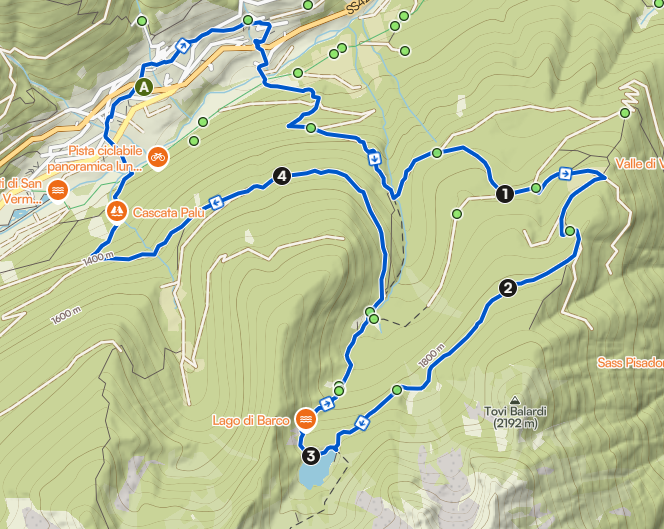
\includegraphics[width=\textwidth]{images/sentieroKomoot.png}
        \caption{Sentiero su Komoot.}
        \vspace{2em} % Aggiunge un po' di spazio tra le due foto
        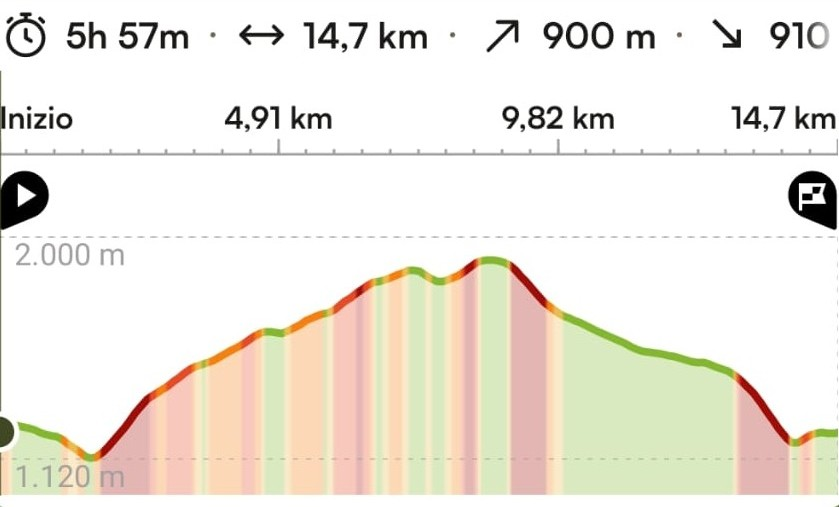
\includegraphics[width=\textwidth]{images/profilo_altimetrico.jpeg}
        \caption{Profilo altimetrico del percorso.}
    \end{subfigure}
    % Didascalia generale per l'intera figura
    \caption{Il sentiero e i dettagli del percorso.}
\end{figure}

% ==========================================================
%  Non ti scordar di me
% ==========================================================
\section{Non ti scordar di me}
\begin{tcolorbox}[colback=yellow!15!white, colframe=yellow!80!black]
\textbf{\textcolor{BurntOrange}{Ricorda: il bivacco è un bene comune. Il suo futuro dipende dal rispetto e dal senso civico dei visitatori. Usalo con cura e lascialo più pulito di come l'hai trovato.}}    
\end{tcolorbox}




\section{Esperienza Personale}
Questa bivaccata è stata molto piacevole e scorrevole, almeno nella sua prima parte. Il paesaggio si è rivelato suggestivo e, fino alla malga, non abbiamo riscontrato alcun tipo di difficoltà. Trattandosi del mese di aprile, la neve era presente ma non particolarmente abbondante, sebbene il sentiero fosse poco frequentato. I veri problemi sono iniziati dopo Malga del Dosso: da quel punto in poi, la neve ha iniziato ad accumularsi in modo significativo, raggiungendo circa un metro di altezza in prossimità dell'ultima salita. Essendo molto fresca, ci ha fatto sprofondare completamente a ogni passo.

Il \textbf{primo giorno} si è concluso con l'arrivo al bivacco, che abbiamo trovato accogliente. La notte è trascorsa in modo molto piacevole: sebbene ci sia voluto del tempo per scaldare completamente la struttura, una volta a regime la temperatura è rimasta gradevole per tutta la notte.

Il \textbf{secondo giorno} abbiamo proseguito su un altro sentiero, scoprendolo molto più scorrevole e agevole rispetto a quello percorso il giorno precedente, il che ci ha permesso di completare il nostro giro in modo soddisfacente.



\section{Alcune foto}

% Sezione Alcune foto

\begin{figure}[htbp!]
    \centering
    % Prima riga: Due foto (QUESTA È LA PRIMA FIGURA)
    \begin{subfigure}[b]{0.45\textwidth}
        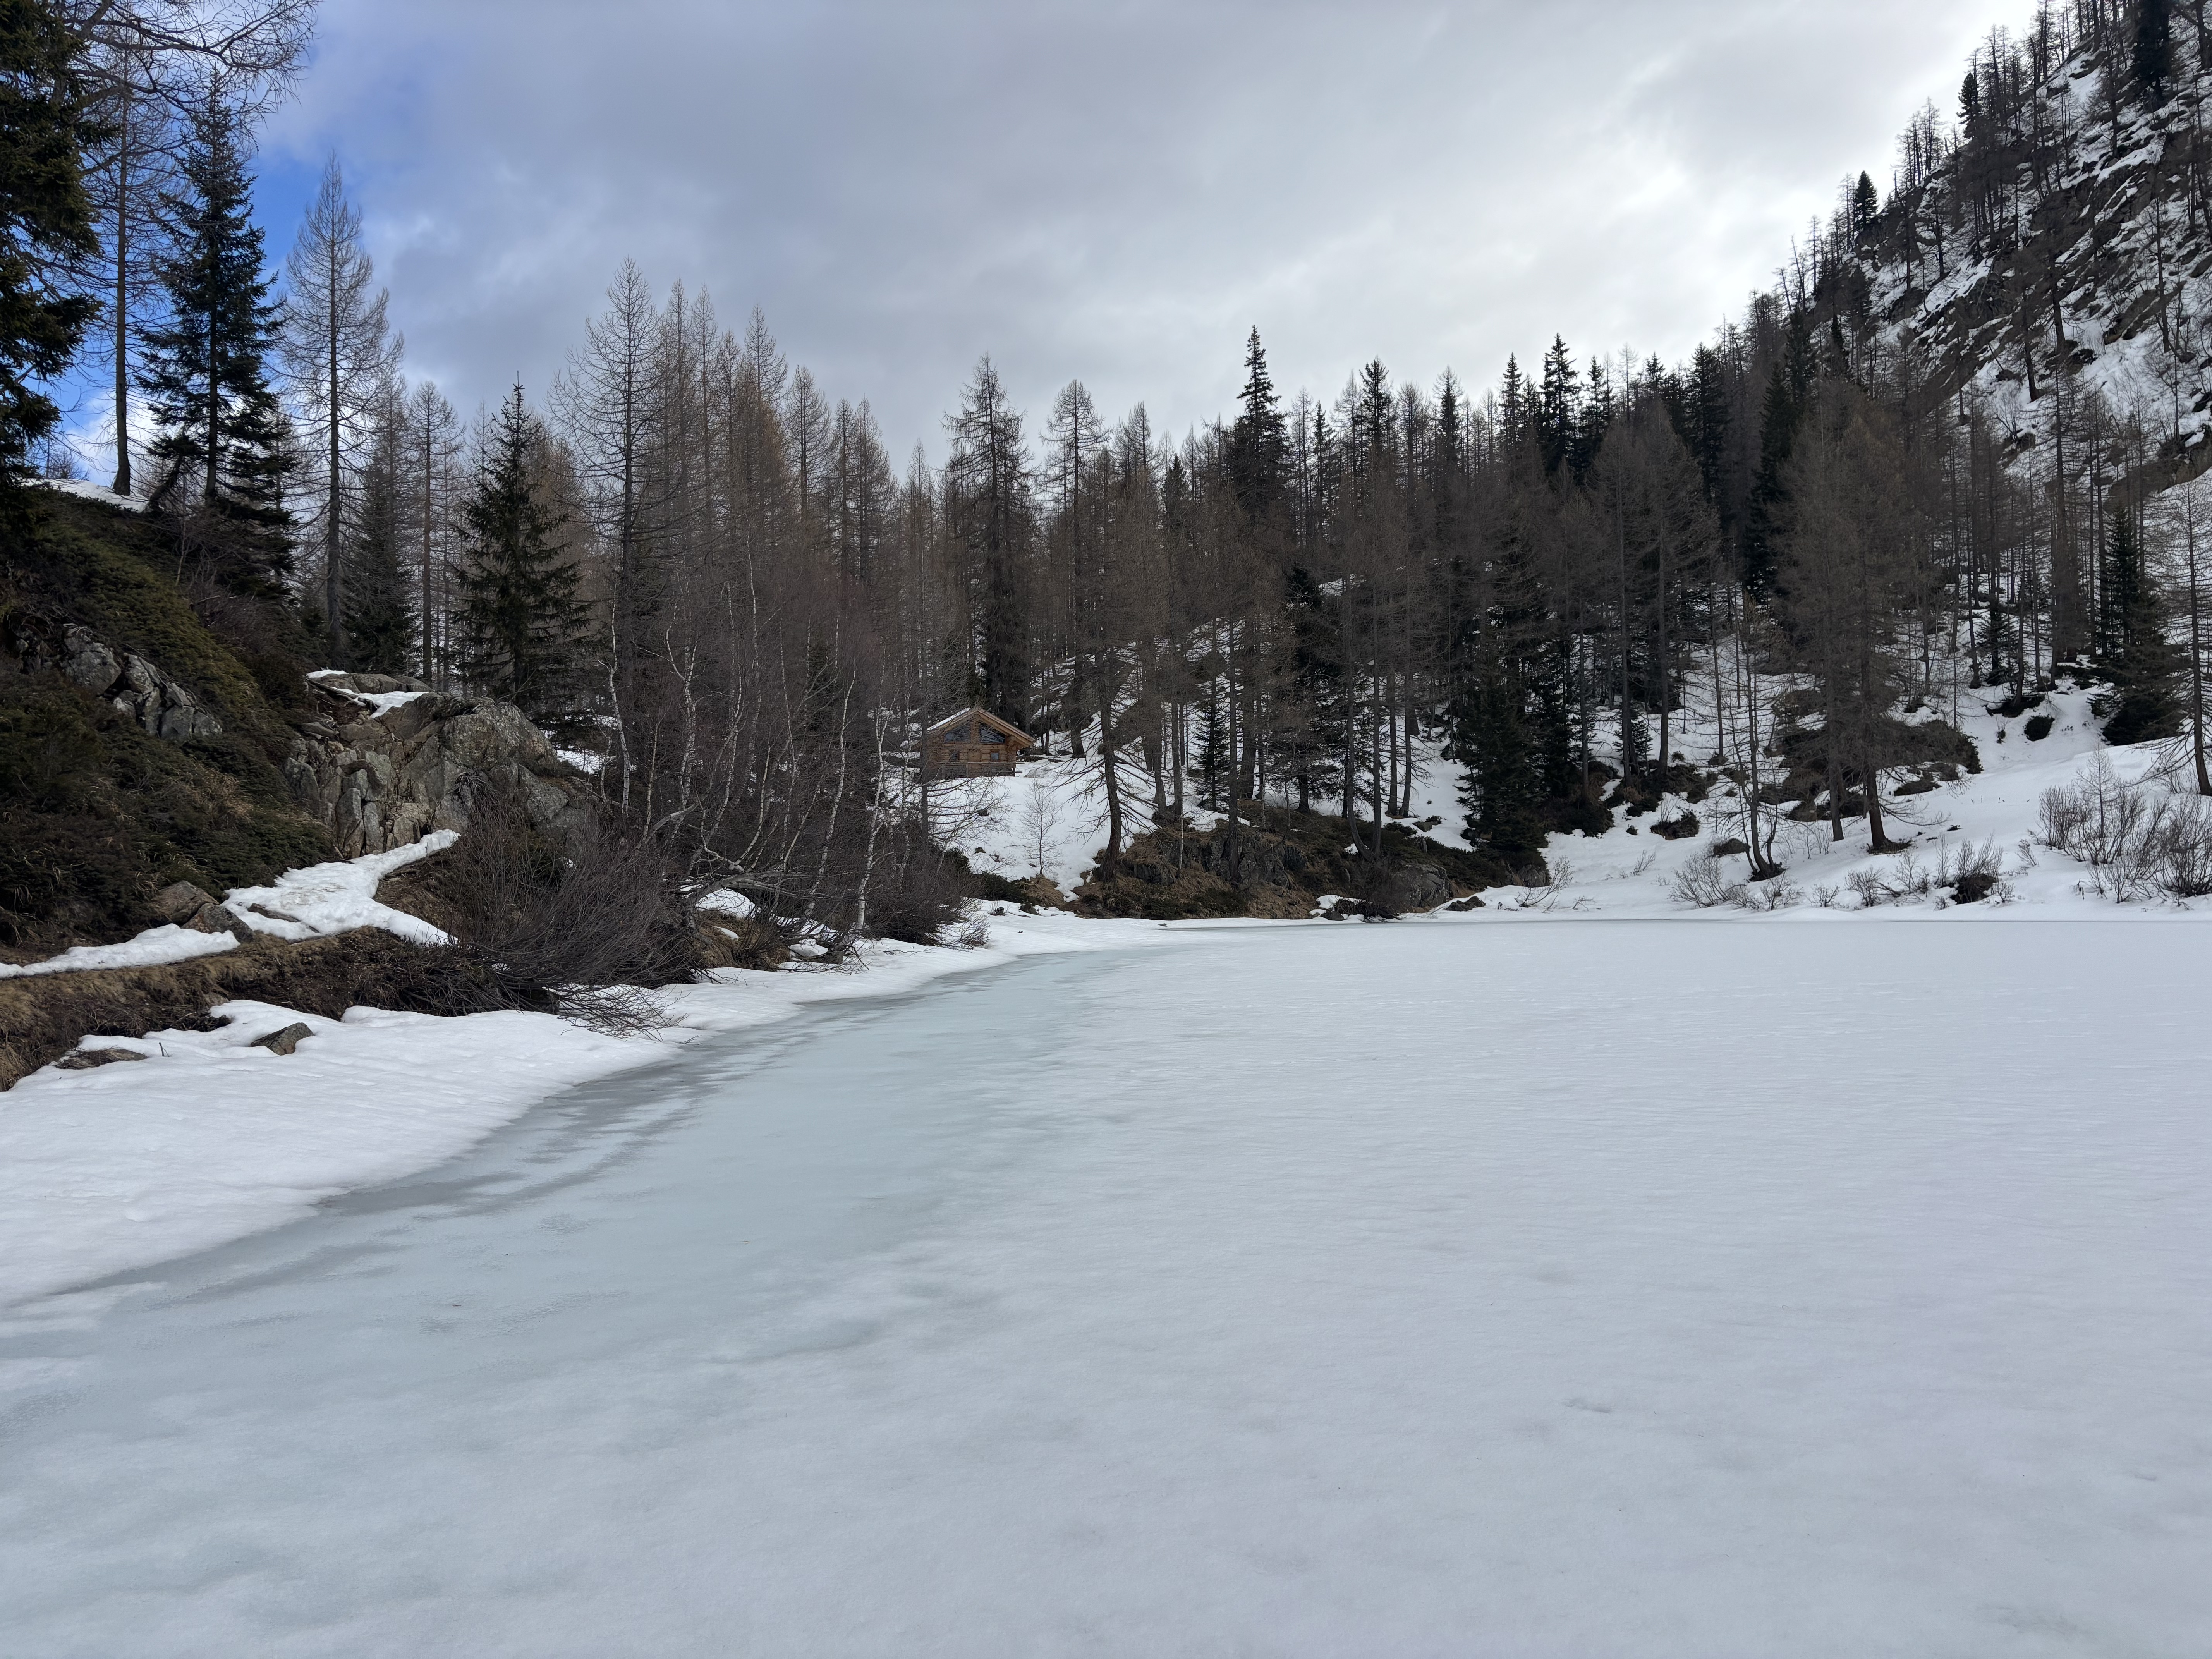
\includegraphics[width=\textwidth]{images/bivacco_lago.jpg}
        \caption{Vista del bivacco con lago ghiacciato.}
    \end{subfigure}
    \hfill
    \begin{subfigure}[b]{0.45\textwidth}
        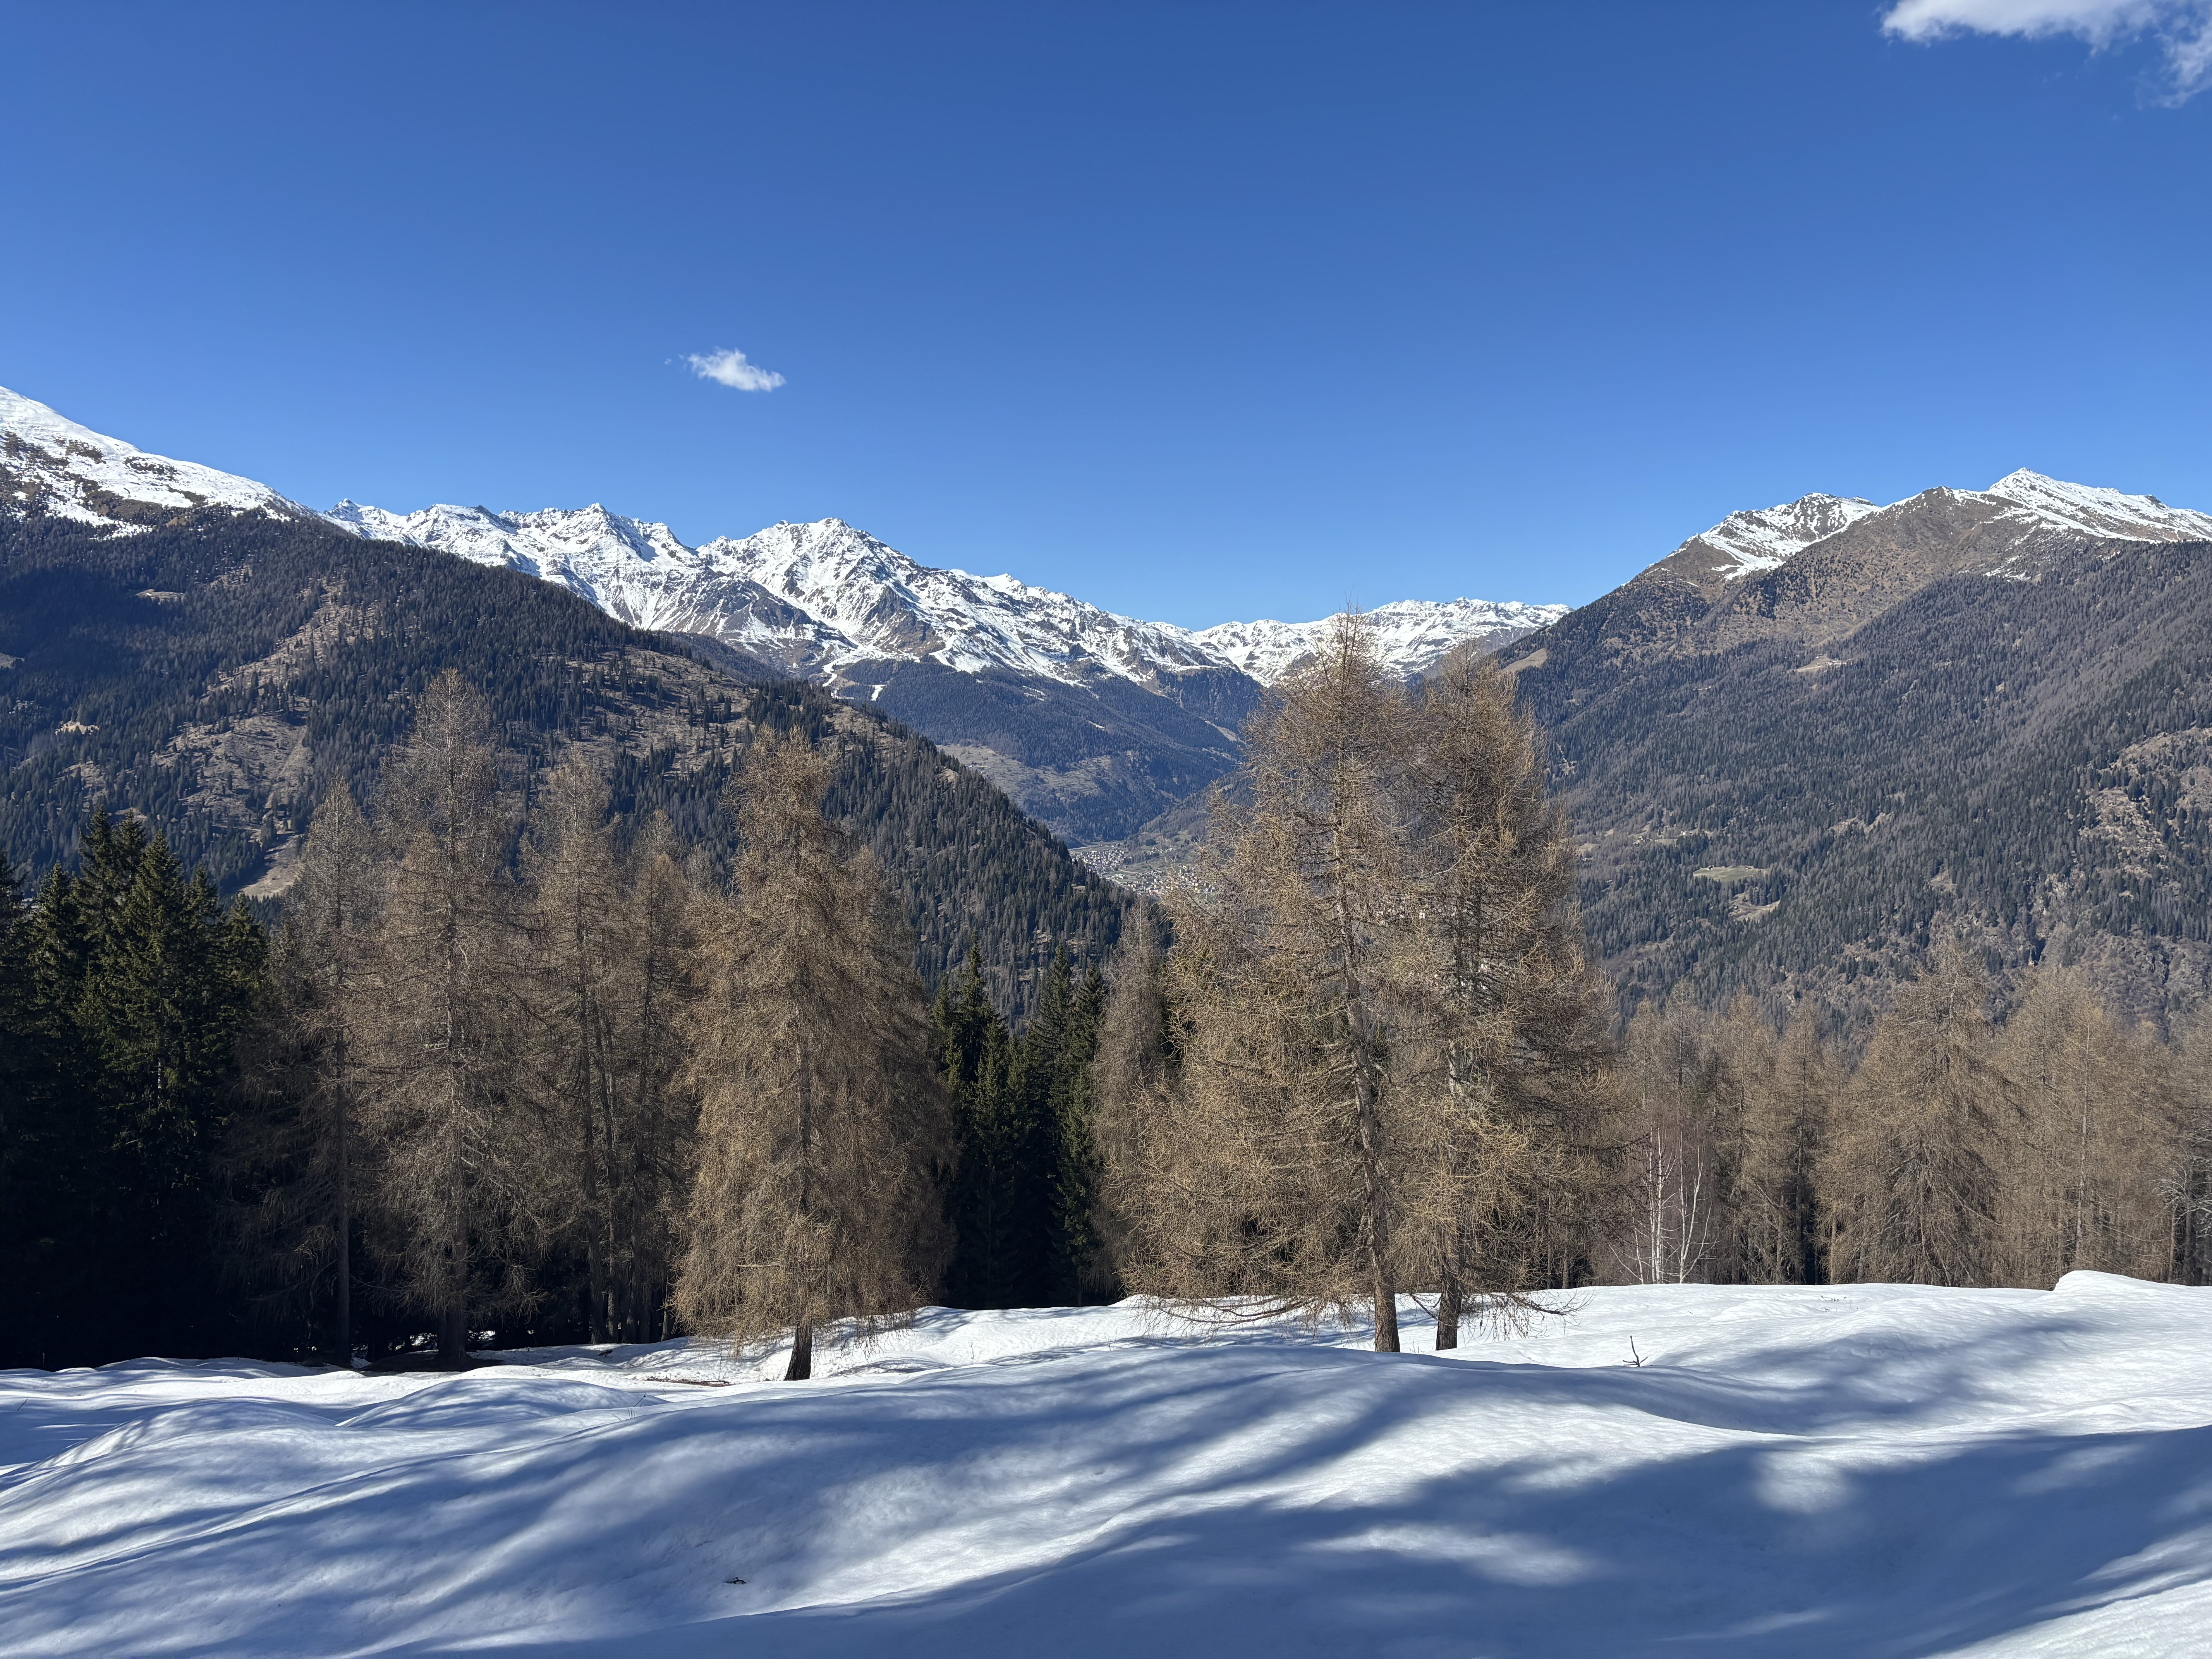
\includegraphics[width=\textwidth]{images/paesaggio.jpg}
        \caption{Paesaggio.}
    \end{subfigure}
    
\end{figure}


\begin{figure}[H]
    \centering
    % Seconda riga: Tre foto (QUESTA È LA SECONDA FIGURA)
    \begin{subfigure}[b]{0.45\textwidth}
        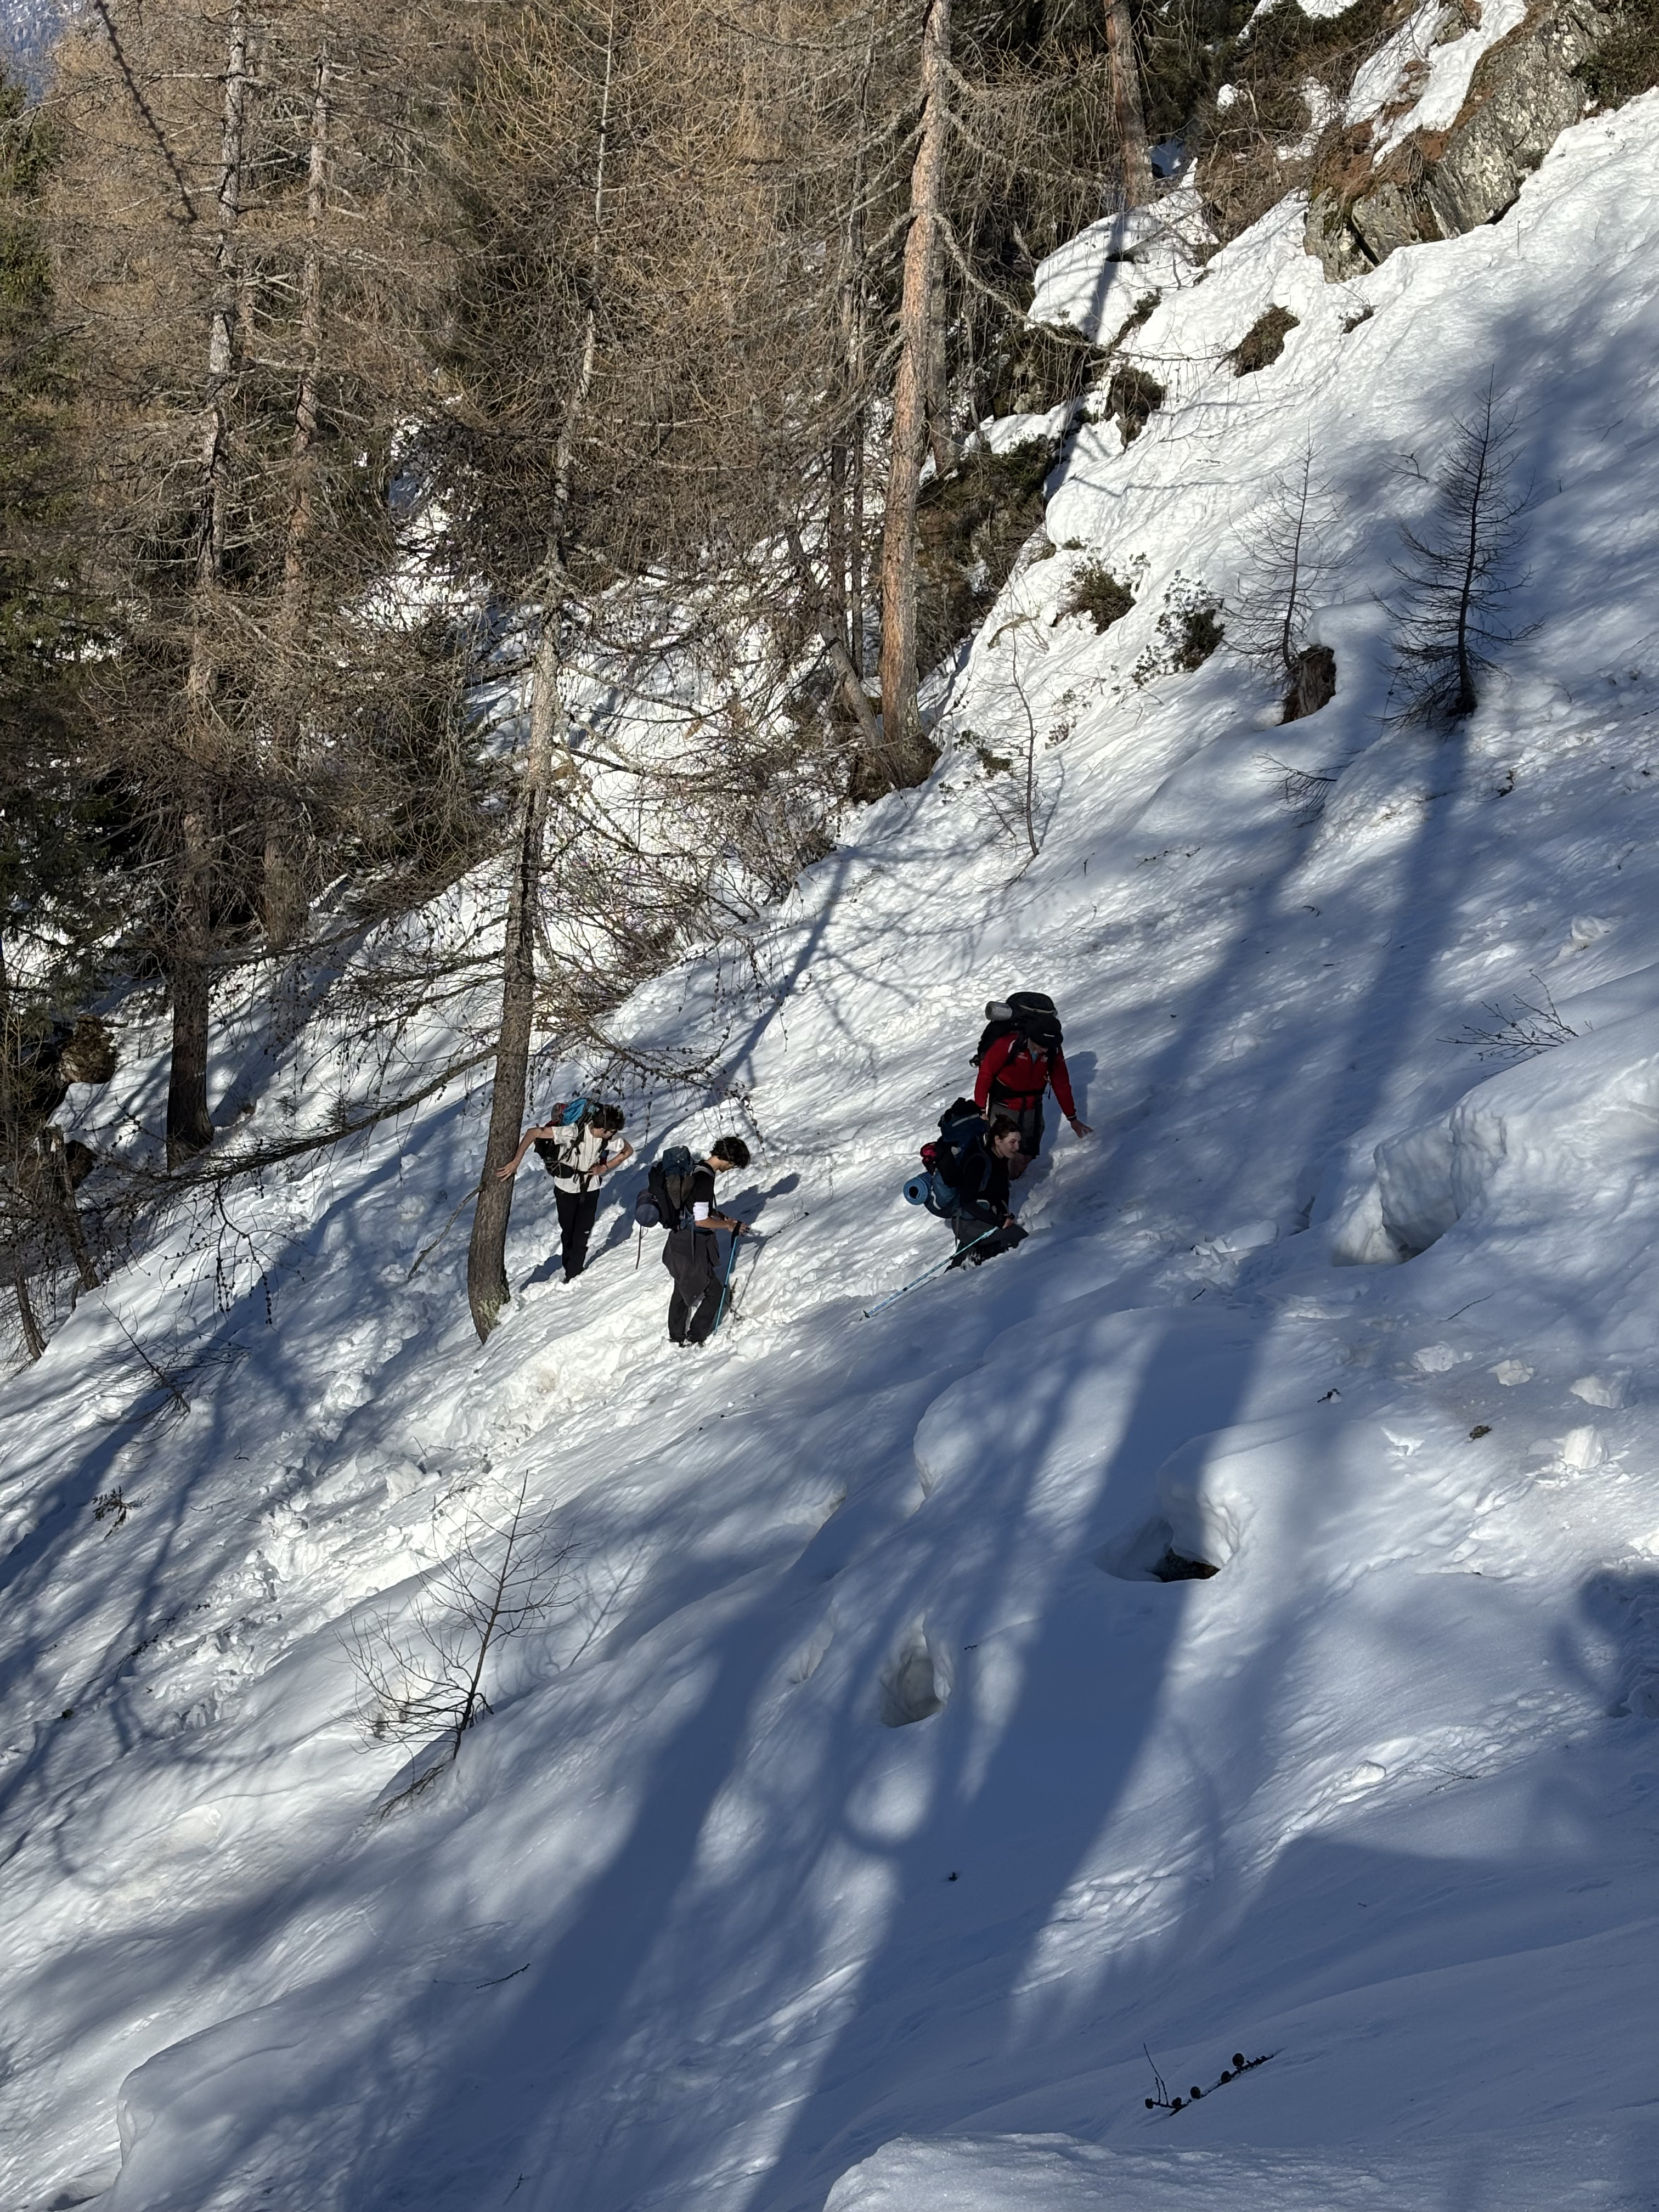
\includegraphics[width=\textwidth]{images/sentiero innevato.jpg}
        \caption{Sentiero innevato.}
    \end{subfigure}
    \hfill
    \begin{subfigure}[b]{0.45\textwidth}
        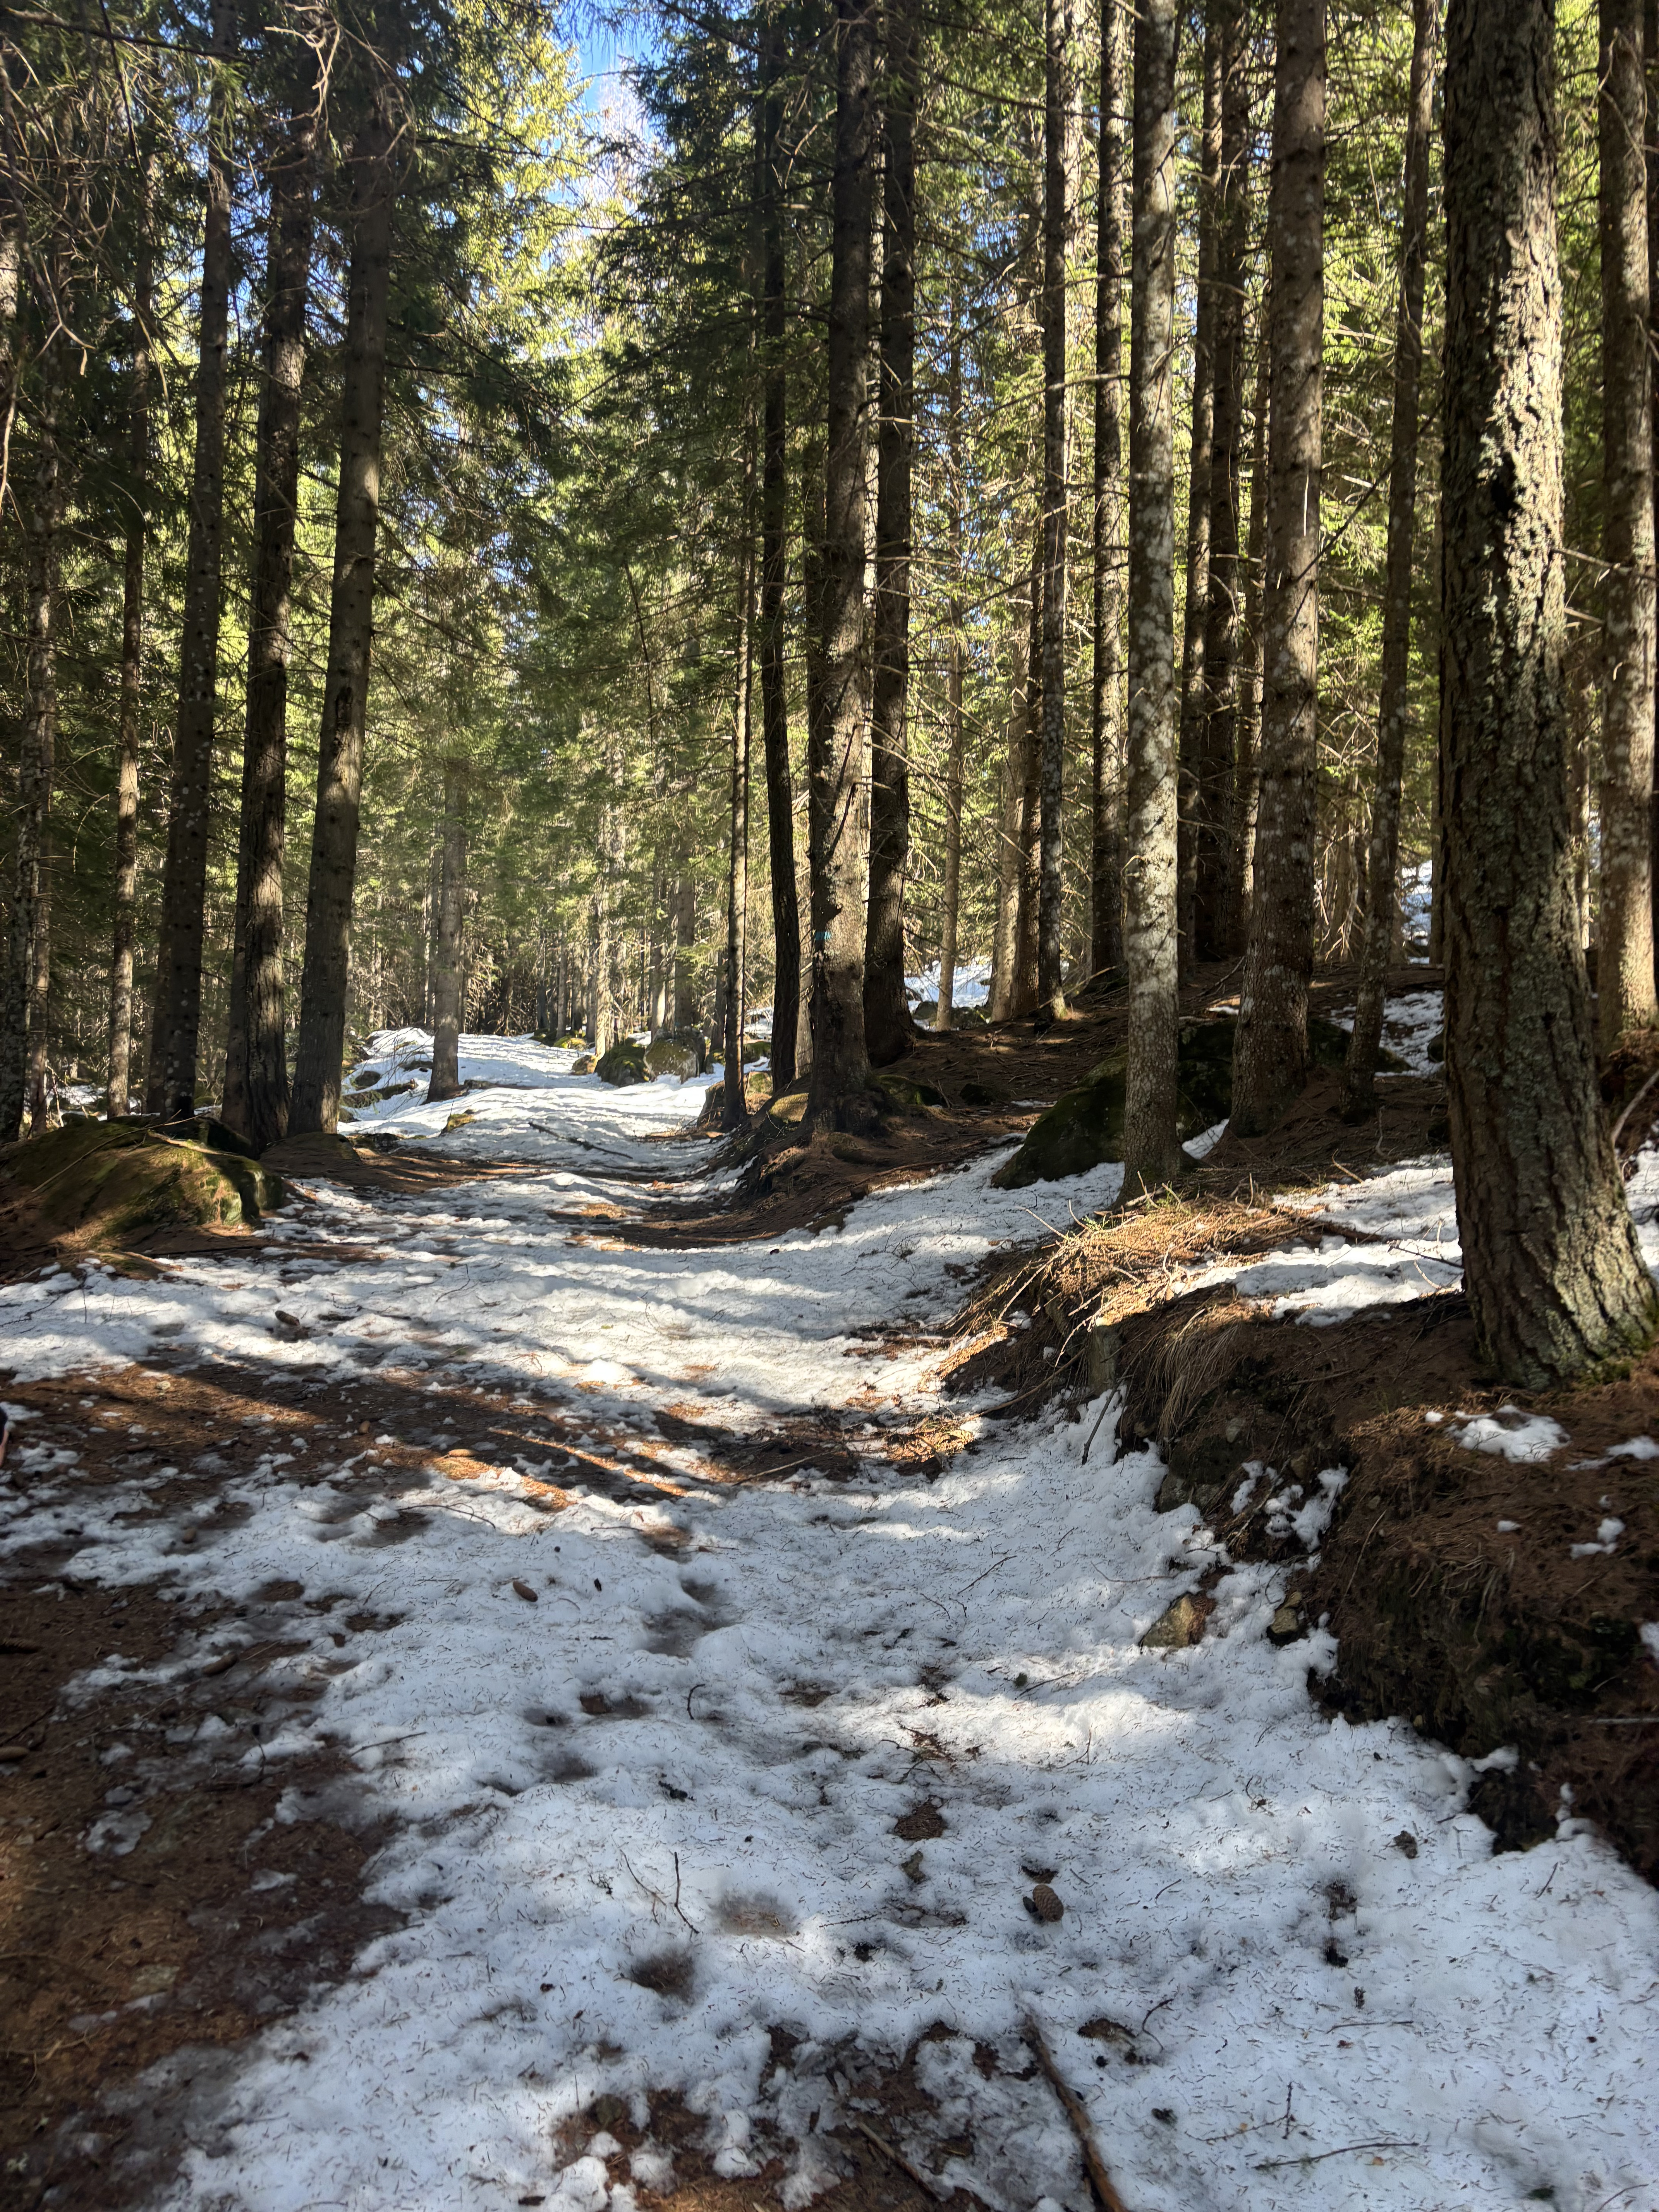
\includegraphics[width=\textwidth]{images/sentiero.jpg}
        \caption{Altro sentiero sul monte.}
    \end{subfigure}
    \hfill
\end{figure}



\clearpage

\section*{Tabella riepilogativa delle caratteristiche}

\begin{tabularx}{\textwidth}{|l|X|}
\hline
\rowcolor{gray!15} \textbf{Caratteristica} & \textbf{Dettaglio} \\
\hline
Regione & Trentino-Alto Adige\\
Provincia / Comune & Trento / Vermiglio \\
Gruppo montuoso & Gruppo della Presanella \\
Quota & 1918 m s.l.m. \\
Apertura & Non gestito, sempre aperto \\
Posti letto effettivi & vari materassi per circa 10 persone \\
Presenze in visita & 6 persone \\
Arredi & Tavolo, panche, stufa  \\
Acqua & \ding{55} - Assente\\
Servizi igienici & \ding{55} - Assente\\
Copertura telefonica & \ding{55} - Poca e solo in determinati punti\\
Manutenzione / proprietà & Pubblico / Comune / Volontari \\
Visitato il & 3-4 Aprile 2026\\
\hline
\end{tabularx}


\end{document}
